% !TEX encoding = UTF-8
% !TEX TS-program = pdflatex
% !TEX root = ../tesi.tex
% !TeX spellcheck = <none>

%**************************************************************
\chapter{L'Azienda}
\label{cap:azienda}
\vspace{20pt}

\section{IKS}

IKS \emph{(Information Knowledge. Supply)} è un'azienda padovana 
fondata, dall'attuale Amministratore Delegato Paolo Pittarello, nel 1999. 

Nell'insieme, IKS unisce figure di alto profilo con lo scopo di 
proporre soluzioni innovative alle richieste di mercato dell'\gls{ict} 
sia italiano che estero. Le soluzioni offerte interessano in particolare 
gli ambiti della sicurezza, dell'infrastruttura e della governance \gls{it}.  

L'azienda è in continua ricerca tecnologica. Investendo sulla formazione 
del proprio personale, IKS si impegna di portare solo valore aggiunto 
al business dei propri clienti. Inoltre, l'Azienda crede fortemente 
nell'innovazione come strumento verso un ambiente digitale comune, 
\gls{agile} e totalmente disponibile. 

Il quartier generale aziendale è a Padova. Inoltre, IKS possiede uffici 
anche nelle seguenti città: Roma, Milano e Trento.

A partire dallo scorso anno (2016), IKS SRL, Kirey SRL, Insirio SPA e 
System Evolution SRL hanno  fondato il Gruppo Kirey. L'obiettivo comune 
delle quattro aziende è l'unione delle competenze complementari e 
garantire un portfolio completo di soluzioni ai clienti attuali e futuri. 

La creazione del Gruppo Kirey è stata guidata dalla Synergo SGR., società di 
\emph{private equity}. Il presidente del nuovo Gruppo commerciale è Vittorio 
Lusvarghi.   

A seguito della creazione del Gruppo, IKS SRL e le restanti tre realtà 
aziendali hanno conservato la propria struttura di governance e management, 
con il fine di garantire la propria continuità gestionale. 

\section{Profilo dell'azienda}
\subsection{Servizi e prodotti offerti}

Nel corso degli anni, IKS si è fatta notare per gli enormi contributi 
innovativi nell'ambito della sicurezza informatica. Tuttavia, essa non 
è limitata a questo ambito. Infatti, gli altri ambiti di applicazione 
sono: infrastruttura e governance IT. 

Di seguito vengono presentati i servizi offerti da IKS per ciascun ambito di 
applicazione:

\begin{itemize}
	\item \textbf{IT Security}\\
	 \begin{itemize}
	 	\item \textbf{Risk analysis e vulnerability assessment}\\ 
	 	È importante garantire la sicurezza dell'infrastruttura 
		informatica nel suo complesso. A questo scopo, IKS offre un 
		servizio orientato alla ricerca di eventuali vulnerabilità e 
		analisi dei rischi a esse collegate;
	 
	 	\begin{figure}[htbp]
	 		\begin{center}
	 			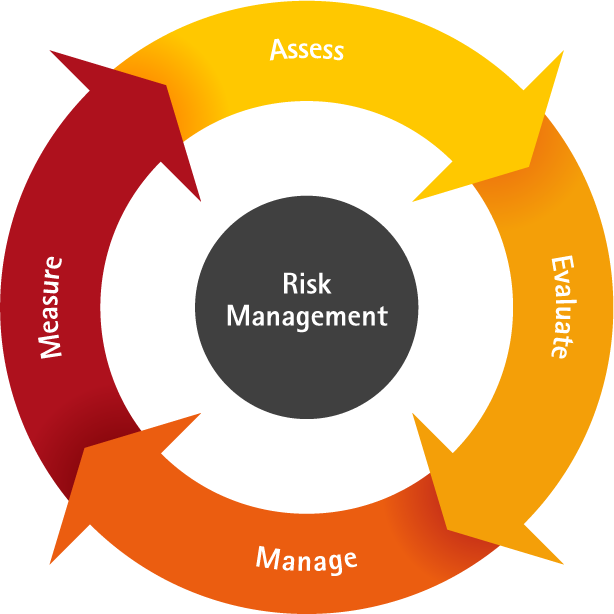
\includegraphics[height=5cm]{risk-management}
	 			\caption{Visione a processo della gestione del 
				 rischio.Immagine tratta da: http://bit.ly/2rh3V0A.}
	 		\end{center}
	 	\end{figure}
	 		 	
		\item \textbf{Audit management}\\
		Le aziende di continuo sono sottoposte a controlli di vario 
		genere; il loro scopo è l'accertamento della 
		regolarità delle aziende con: certificazioni, normative, bilanci 
		ed ecc. IKS offre un servizio di supporto per le aziende con 
		il fine di agevolare le attività di \emph{auditing} 
		ed eventualmente per migliorare i loro processi interni;
		\begin{figure}[htbp]
			\begin{center}
				\hspace{3em}
				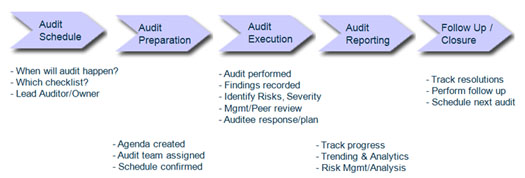
\includegraphics[height=3.5cm]{audit-management}
				\caption{Flusso di lavoro durante lo 
				svolgimento di un \emph{audit}.
				Immagine tratta da: http://bit.ly/2rdFhfv.}
			\end{center}
		\end{figure}
	
	 	\item \textbf{Difesa perimetrale}\\ 
	 	Sempre in ambito della sicurezza è importante prendere le 
		giuste misure per garantire a priori uno specifico livello 
		di sicurezza e limitare a zero le intrusioni dall'esterno 
	 	di un'infrastruttura IT aziendale. A questo scopo, IKS offre 
		un'insieme di soluzioni orientare al monitoraggio degli 
		accessi a sistemi aziendali, dei permessi sulle operazioni 
	 	che un utente può effettuare, e molto altro;
	 	\begin{figure}[htbp]
	 		\begin{center}
	 			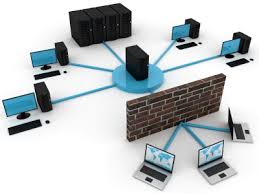
\includegraphics[height=4cm]{firewall}
	 			\caption{Visione grafica del concetto di difesa 
				perimetrale. Immagine tratta da: 
				http://bit.ly/2s834O2.}
	 		\end{center}
	 	\end{figure}	 	
	 \end{itemize}	
	\item \textbf{IT Infrastructure}\\
	 \begin{itemize}
	 	\item \textbf{Business continuity}\\
	 	In ambito bancario, le infrastrutture informatiche sono molto 
		complesse. La manutenzione delle infrastrutture informatiche non è 
		semplice. La sfida più difficile è garantire che questi sistemi siano 
		operativi al 100\%. Una simile percentuale nella pratica è 
		impossibile. IKS con il proprio gruppo di esperti sono alla 
		continua ricerca di soluzioni per incrementare la percentuale 
		di continuità operativa di questi sistemi. Infatti, le 
		soluzioni offerte dall'azienda sono orientate nel concreto 
		all'infrastruttura del cliente richiedente supporto;
	 	\begin{figure}[htbp]
	 		\begin{center}
	 		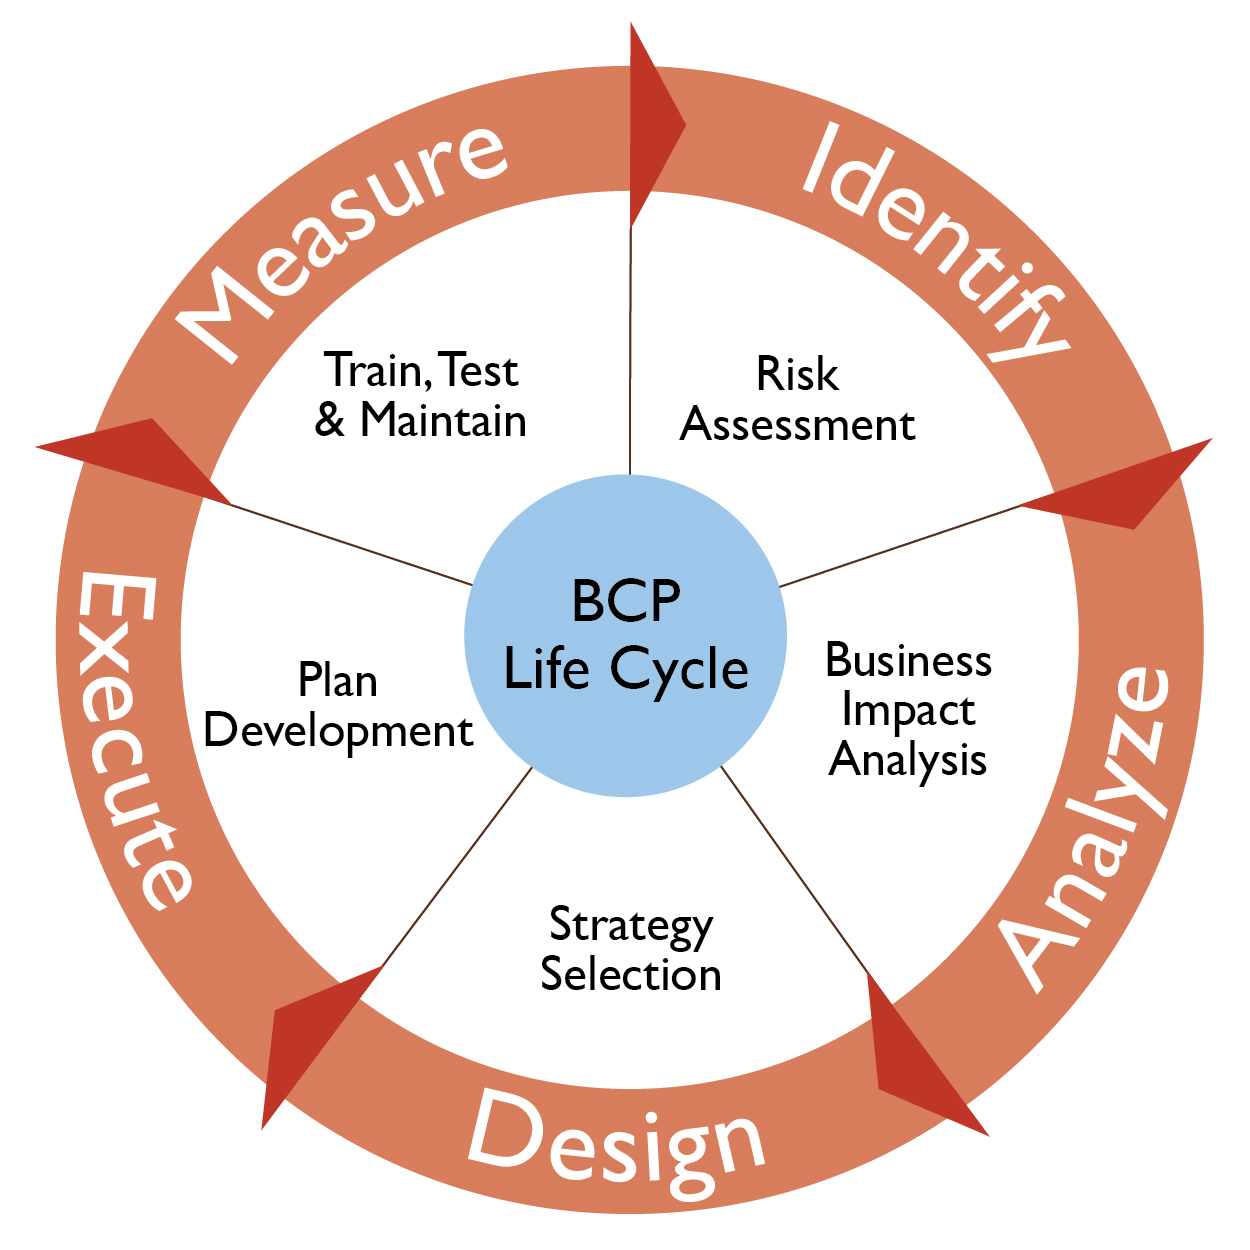
\includegraphics[height=6cm]{business-continuity}
				\caption{Visione del ciclo di vita del 
				processo di \emph{business continuity}. 
				Immagine tratta da: http://bit.ly/2qvCmgP.}
			\end{center}
			\end{figure}

%\newpage
		\item \textbf{Virtualization technology}\\
		 Ogni prodotto software di business per portare valore aggiunto 
		 deve essere eseguito. Eseguire un prodotto software per server 
		 fisico richiede la disponibilità di un cospicuo numero di server. 
		 A questo scopo la tecnologia di virtualizzazione permette la 
		 creazione di server virtuali che eseguono programmi e questi 
		 vengono eseguiti da server fisici. I benefici di una simile 
		 infrastruttura è l'ottimizzazione delle risorse di calcolo, 
		 agilità di gestione e sicurezza. Alcune delle soluzioni di 
		 virtualizzazione offerte da IKS sono: VMWare, RHEV ed ecc. 
		 Un'evoluzione della tecnologia di virtualizzazione è il \emph{Cloud}. 
		 In questo ambito, IKS propone soluzioni di migrazione e supporto 
		 verso il Cloud dell'infrastruttura IT classica di un'azienda;  
		 \begin{figure}[htbp]
			\begin{center}
				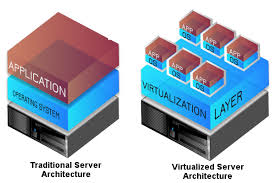
\includegraphics[height=4cm]{virtualization}
				\caption{Vista a confronto: ambiente 
				server bare metal e virtualizzato. 
				Immagine tratta da: http://bit.ly/2qvtLLk.}
			\end{center}
		 \end{figure}
 	\end{itemize}

	\item \textbf{IT Governance}\\
	\begin{itemize}
		\item \textbf{Service management}\\
		Un servizio informatico di business, a causa della sua criticità,
		richiede costante attenzione. Il monitoraggio del servizio 
		informatico presenta la necessità di enormi investimenti 
		economici. IKS offre piani di gestione per soddisfare 
		anche i più esigenti clienti;
	    
	    \begin{figure}[htbp]
	    	\begin{center}
	    		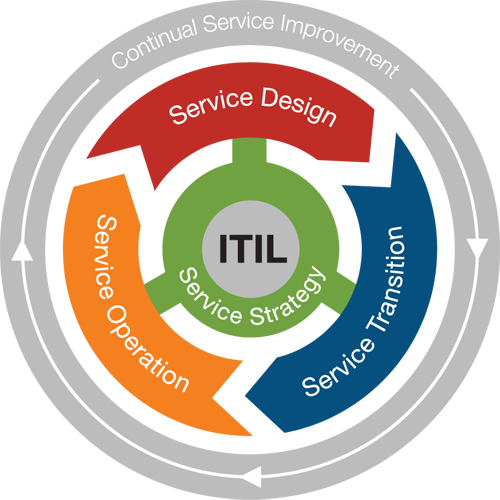
\includegraphics[height=6cm]{itil}
	    		\caption{Visione della gestione di servizio in 
				prospettiva del \gls{framework} ITIL. Immagine tratta da: 
				http://bit.ly/2qvNryk.}
	    	\end{center}
	    \end{figure}
	    
		\item \textbf{Application and performance monitoring}\\ 
		Ogni prodotto software ha il proprio specifico ciclo di vita. 
		Concluso il ciclo di sviluppo, il prodotto è rilasciato in 
		produzione. La seconda parte del ciclo di vita di un prodotto 
		software è la manutenzione. Il monitoraggio di un applicativo 
		è importante per avere una costante visione dello stato del 
		prodotto e prevenire eventuali esigenze di manutenzione generica 
		oppure di basso profilo a livello di codice sorgente. In questo 
		dominio, grazie a partnership strategiche, IKS offre soluzioni 
		mirate a garantire la miglior possibile esperienza di 
		monitoraggio applicativo;
		\begin{figure}[htbp]
			\begin{center}
				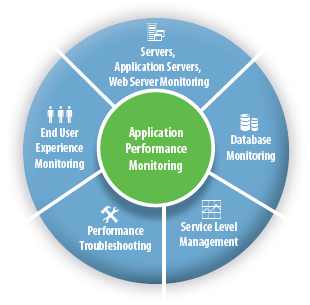
\includegraphics[height=7cm]{application-performance-monitoring}
				\caption{Oggetto del monitoraggio sono: gli utenti, i server, 
					     le applicazioni ed ecc. Immagine tratta da: 
						 http://bit.ly/2v3MuE2.}
			\end{center}
		\end{figure}
		
		\item \textbf{System and networking management}\\
		Gestire sistemi e reti informatiche è un compito complesso. 
		L'utilizzo di strumenti adeguati permette di semplificare il 
		lavoro e garantisce un stato consistente del sistema nel tempo. 
		Le soluzioni che IKS offre sono orientate alla flessibilità e 
		facilità d'uso dei prodotti offerti in questo contesto;
	\end{itemize} 
	\item \textbf{Innovation \& Project} \\
	\begin{itemize}
		\item \textbf{Architetture applicative distribuite}\\
		I sistemi informatici diventano sempre più di natura 
		distribuita. IKS offre in questo ambito soluzioni architetturali 
		orientate a microservizi, utilizzando le ultime tecnologie 
		orientate alla containerizzazione e orchestrazione di container; 
		
		\item \textbf{Sviluppo di applicazioni cloud native}\\
		È comune sentire parlare di cloud. Le classiche 
        architetture applicative non riescono a beneficiare della 
		flessibilità del cloud, perché in organizzazione e struttura 
		non sono scalabili e sono difficilmente modularizzabili. Applicazioni
		che vengono gestite nel complesso come un'unica unità prendono il nome di 
		monolite. La diretta conseguenza di una simile organizzazione è 
		il carattere statico e poco flessibile dell'applicazione. Paradigmi nuovi, 
		per la messa in esercizio di applicazioni, mancano l'intigrazione 
		con architetture software tradizionali. Per questo motivO, 
		le applicazioni devono essere sviluppate fin dal principio con 
		un'architettura orientata al Cloud. Una buona guida, di sviluppo 
		di applicazioni orientate al Cloud, è la segeunte: \textit{Twelve Factor-Factor App}.,
		Heroku, servizio  PaaS per applicazioni cloud native, promuove 
		continuamente l'importanza dei 12 principi alla base della filosofia 
		\emph{cloud native}. In questa direzione IKS propone servizi di sviluppo 
		di applicazioni di business orientate all'affidabilità, resilienza, 
		scalabilità orizzontale ed ecc.
		
		\begin{figure}[htbp]
			\begin{center}		
			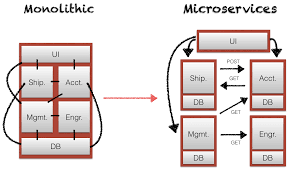
\includegraphics[height=4cm]{monolith-microservice}
			\caption{Visione architetturale a monolite e 
				microservizi a confronto. 
				Immagine tratta da: http://bit.ly/2rh1niY.}
			\end{center}
			\end{figure}
			\end{itemize} 
		\end{itemize}

La clientela tipica di IKS sono le aziende operanti nei seguenti ambiti: 
pubblica amministrazione, bancario, assicurativo e servizi. 

Una lista dettagliata delle referenze può essere consultata sul sito
di IKS (\url{https://www.iks.it/referenze.html}).

\subsection{Struttura organizzativa}

Ad oggi, IKS conta più di 100 dipendenti. La sua organizzazione interna è 
riassunta nel diagramma in \textbf{Figura 1.9}.

In seguito, descrivo le unità operative che costituiscono il nucleo 
decisionale dell'azienda. Queste unità sono:
\begin{itemize}
	\item \textbf{Direzione}\\ 
	Definisce gli orientamenti e le politiche aziendali, gli 
	obiettivi per la qualità, riesamina periodicamente il sistema di 
	qualità e gestisce il piano di formazione dei dipendenti in funzione 
	alle esigenze e motivazioni personali;
	
	\item \textbf{Direzione Commerciale}\\
	Definisce le politiche commerciali, gli obiettivi e le risorse 
	necessarie. Promuove i servizi e prodotti dell'azienda. Gestisce i 
	clienti, i fornitori e le offerte contrattuali;
	
	\item \textbf{Direzione tecnica o Operation}\\
	Supporta la Direzione Commerciale nella valutazione commerciale di 
	prodotti e/o offerte dal punti di vista tecnico. Gestisce a livello 
	tecnico i progetti e servizi. Pianifica le risorse necessarie per 
	i prodotti/servizi. Verifica lo stato del prodotto/servizio offerto;	
	
	\item \textbf{Amministrazione \& Finanza}\\
	Gestisce la documentazione di progetto, su coordinamento della direzione 
	commerciale e tecnica. Gestisce l'archiviazione della documentazione;
	
	\item \textbf{Acquisti}\\
	Su coordinamento della Direzione, gestisce i fornitori di prodotti e 
	servizi. Gestisce il processo di acquisizione di nuovi prodotti o 
	servizi. Il processo di acquisizione è guidato dalle necessità 
	interne aziendali oppure da quelle dei clienti;
	
	\item \textbf{Assicurazione Qualità}\\
	È a stretto contatto solo con la Direzione. Gestisce il piano di 
    qualità, coordina le attività di ispezione, misura e stima il livello 
	della qualità aziendale;
	
	\item \textbf{Business Unit (BU)}\\
	Gestisce i progetti o servizi concordati con il Cliente. Rendiconta 
	direttamente alla Direzione Tecnica e gestisce l'emissione delle 
	fatture verso il Cliente. 
\end{itemize}


\begin{figure}[htbp]
	\begin{center}
		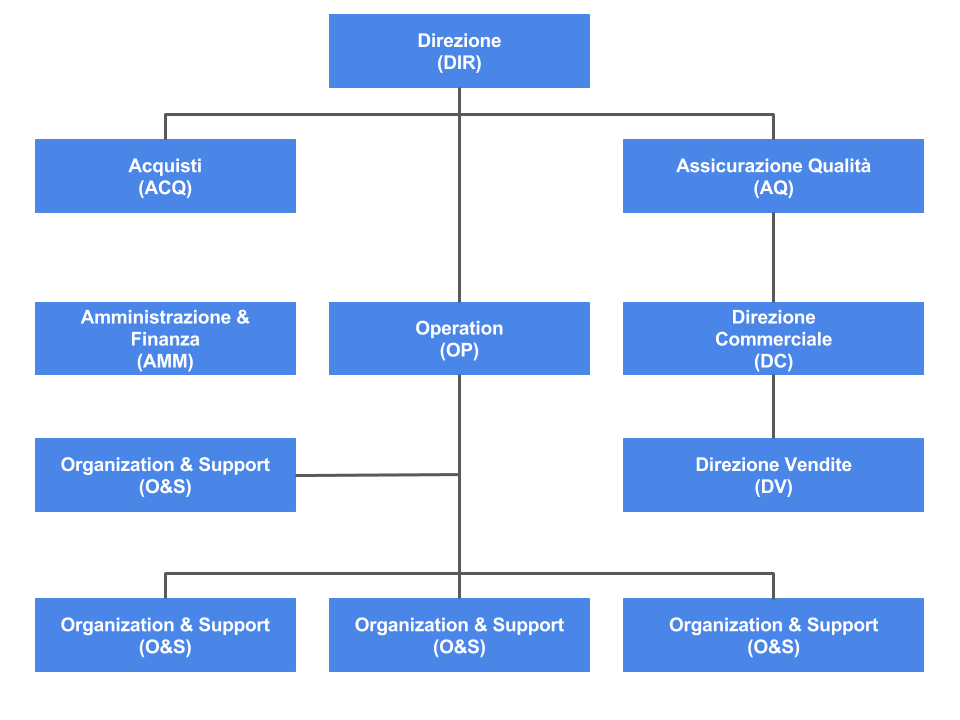
\includegraphics[height=8cm]{organigramma}
		\caption{Organigramma aziendale}
	\end{center}
\end{figure}



\subsection{Processi aziendali}

IKS, a partire dal 2003, è certificata UNI EN ISO 9001. Questo certifica che 
l'azienda cura molto la qualità del proprio lavoro. Infatti, il miglioramento 
continuo permette all'azienda di rimanere competitiva e consolidare 
la propria posizione di leader sul mercato del ICT italiano. Riporto, di seguito, 
alcuni obiettivi di qualità dell'azienda:

\begin{itemize}
	\item Mantenere e aumentare il livello di soddisfazione del Cliente;
	\item Operare in modo efficiente ed efficace per soddisfare i requisiti 
		  contrattuali, norme e regolamenti;
	\item Monitorare i propri processi per: garantire azioni correttive 
	      tempestivamente e permettere un comportamento pro attivo, 
	      anticipare i bisogni e predire le risorse aziendali necessarie 
	      prima dell'effettivo bisogno; 
	\item Assicurare una adeguata formazione al Personale.
\end{itemize}


Il Cliente copre un ruolo importante nella quotidinità di IKS. Infatti, 
l'azienda cerca di coinvolgere i propri clienti il più possibile., questo 
è necessario per comprendere meglio i bisogni attuali del cliente e 
cogliere esigenze future. 
In azienda, il passo successivo alla formalizzazione del bisogno del 
Cliente segue un'attività di analisi dei requisiti. L'obiettivo 
dell'attività è la dettagliata comprensione del contesto applicativo, 
quali sono le parti interagenti e quali possono essere i rischi, durante 
l'attività di progetto, per implementare i bisogni del Cliente.

A progetto concluso, il Cliente valuta criticamente la soluzione 
presentata. La valutazione, eventualmente, coinvolge un reclamo. Questo 
è rivolto alla Direzione dell'Azienda.

IKS organizza il proprio lavoro per processi: primari, direttivi e di supporto. 
Ciascuna categoria di processo definisce delle responsabilità e compiti. 
Per esempio, i processi organizzativi interessano le attività per: definire la politica 
e strategia aziendale, pianificare e allocare le risorse, riesaminare la gestione del 
sistema di qualità. Invece, i processi primari ricoprono attività che garantiscono 
un diretto ricavo economico per l'azienda e danno un valore aggiunto al prodotto o 
servizio fornito. Esempi di attività in questa categoria sono: proporre offerte 
commerciali ai clienti, progettare e sviluppare prodotti software, erogare servizi IT. 
L'ultima categoria di processi sono i processi di supporto. Le consone attività giornaliere 
riguardano: gestire le risorse umane, l'infrastruttura 
e gli ambienti di lavoro., monitorare e analizzare la qualità aziendale. 

In \textbf{Figura 1.10} segue una presentazione dello schema organizzativo 
utilizzato dall'Azienda, durante il ciclo di vita di un progetto.

\begin{figure}[htbp]
	\begin{center}
		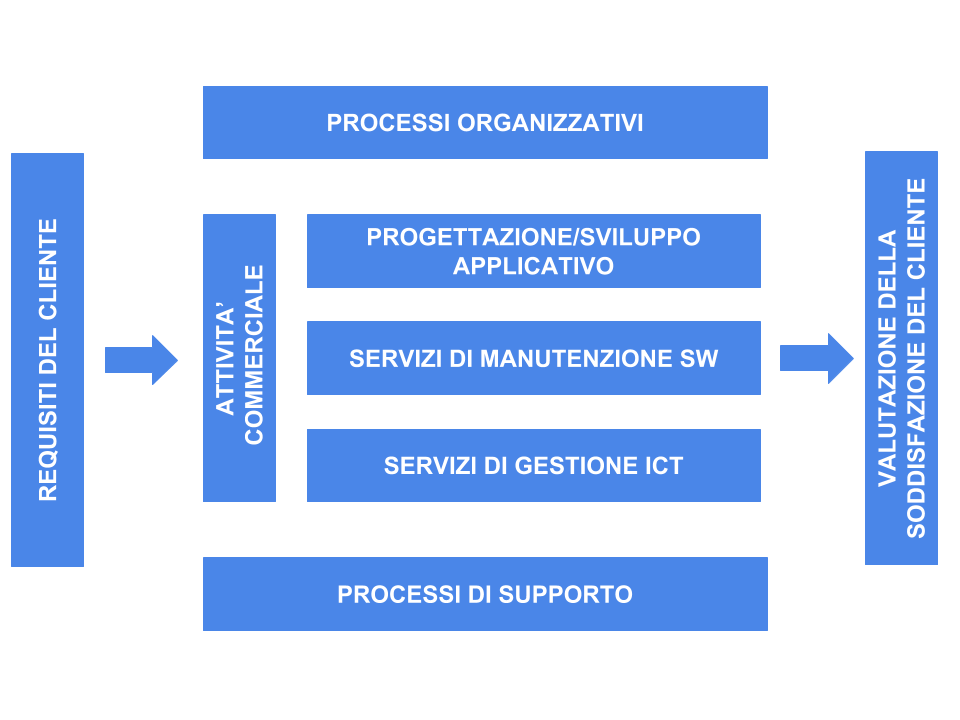
\includegraphics[height=7cm]{relazione-responsabilita}
		\caption{Rappresentazione grafica del coinvolgimento del 
			Cliente e i corrispettivi livelli degli interventi del gruppo 
			commerciale, tecnico, direzionale e di supporto nella gestione 
			di un'offerta di progetto.}
	\end{center}
\end{figure}


Periodicamente, il responsabile della qualità, incaricato della Direzione, attua 
attività d'ispezione. L'obiettivo dell'attività è il controllo del livello di qualità
fornita dai dipendenti aziendali. A posteriori, segue un'attività di 
analisi e misura dei livelli di qualità organizzati per BU, servizio e 
prodotto offerto da IKS.




\section{Rapporto con l'innovazione}
L'innovazione è il processo di gestione dell'intero ciclo di vita di un'idea. 
L'obiettivo è: portare un miglioramento di processo aziendale, di prodotto e/o 
di servizio. Le conseguenze dirette del miglioramento sono: valore aggiunto, per 
l'azienda, in termini di rientro economico e soddisfare un 
bisogno, per il Cliente, in modo efficace ed efficiente. 

L'approccio innovativo induce l'utilizzo dell'informazione, della creatività e 
dello spirito d'iniziativa per raccogliere maggior valore aggiunto dalle risorse a 
disposizione. L'azienda utilizza l'innovazione per soddisfare in modo pro attivo 
le richieste del Cliente. Questo principio è pienamente il linea con la strategia 
di qualità aziendale: \textit{client first}.

La modalità di innovazione di IKS è un approccio incrementale. Inizialmente 
l'azienda cerca di soddisfare i bisogni principali e raggiungere il prima 
possibile gli obiettivi minimi pre-fissati. In seguito, l'azienda migliora 
la propria offerta mediante incrementi continuativi di dettaglio. 

Per supportare l'innovazione, IKS ha creato una cultura aziendale che permette 
ai propri dipendenti di scambiarsi idee, sperimentare, imparare in gruppo e mettere in 
atto la propria creatività. Non manca la comunicazione con i propri responsabili. 
Questi sono i primi a motivare di continuo le risorse umane a loro disposizione. 
Il dialogo dipendente-responsabile non è verticale. La cultura aziendale in questa 
direzione è molto drastica: favorire uno scambio di idee in modo che esso sia  
equo, semplice e non orientato alle gerarchie aziendali. 

In questo contesto, per l'intera durata del mio periodo di stage e dopo un 
primo momento di ambientamento, io ho beneficiato molto del clima aziendale. 
Infatti, non è mancato il libero confronto con il tutor aziendale, il quale ha  
mostrato disponibilità e apertura al mio spirito d'iniziativa. Sempre mio tutor 
aziendale ha supportato me in ogni scelta decisionale che io abbia motivato e 
ritenuto significativa per il beneficio del mio progetto. 

Le idee sono una parte del processo di gestione dell'innovazione: la realtà è 
molto più complessa. IKS non possiede un effettivo processo di gestione a 
livello aziendale. Questo viene gestito da un gruppo di persone con competenze 
trasversali e a livelli organizzativi differenti. 

%\begin{figure}[htbp]
%   \begin{center}
%	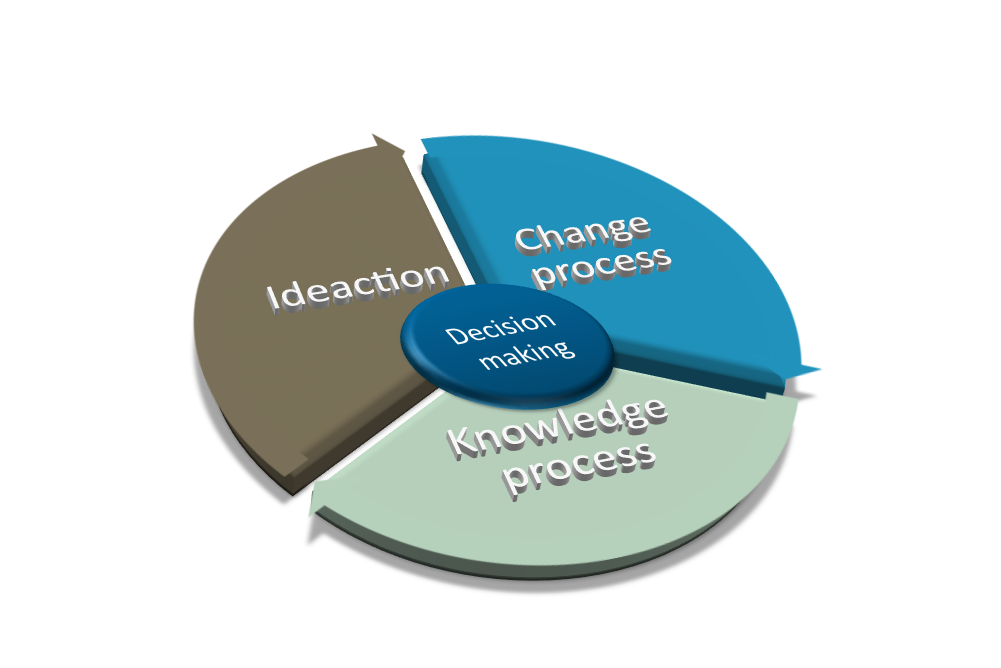
\includegraphics[height=5cm]{innovation-management}
%	\caption{Il legame attivo tra innovazione e il processo del cambiamento 
%	e gestione della conoscenza. Immagine tratta da: http://bit.ly/2qty3XD.}
%   \end{center}
%\end{figure}

\newpage 